\documentclass[9pt,a4paper]{article}

\usepackage[margin=6mm]{geometry}
\usepackage[utf8]{inputenc}
\usepackage[T1]{fontenc}
\usepackage{lmodern}
\usepackage{graphicx}
\usepackage[table]{xcolor}
\usepackage{tabularx}
\usepackage{array}
\usepackage{booktabs}
\usepackage{enumitem}
\usepackage[most]{tcolorbox}
\usepackage{tikz}
\usepackage{ragged2e}
\usepackage{multicol}

\pagestyle{empty}
\setlength{\parindent}{0pt}
\setlength{\parskip}{0pt}
\setlength{\tabcolsep}{3pt}
\renewcommand{\arraystretch}{1.08}
\graphicspath{{paper_assets/}}
\sloppy

\definecolor{PosterInk}{HTML}{17324D}
\definecolor{PosterBlue}{HTML}{0D6EA6}
\definecolor{PosterTeal}{HTML}{13857B}
\definecolor{PosterOrange}{HTML}{DD7A2F}
\definecolor{PosterRed}{HTML}{B24D57}
\definecolor{PosterLine}{HTML}{D7E0EA}
\definecolor{PosterSoft}{HTML}{F5F9FC}

\newtcbox{\flowchip}{
    on line,
    colback=white,
    colframe=PosterLine,
    boxrule=0.45pt,
    arc=1.8mm,
    left=1.2mm,
    right=1.2mm,
    top=0.8mm,
    bottom=0.8mm,
    boxsep=0pt
}

\newtcolorbox{metcard}[1]{
    enhanced,
    colback=#1,
    colframe=#1,
    boxrule=0pt,
    arc=2.1mm,
    left=1.8mm,
    right=1.8mm,
    top=1.2mm,
    bottom=1.2mm,
    boxsep=0pt
}

\newtcolorbox{posterbox}{
    enhanced,
    colback=white,
    colframe=PosterLine,
    boxrule=0.55pt,
    arc=2.2mm,
    left=1.7mm,
    right=1.7mm,
    top=1.4mm,
    bottom=1.4mm,
    boxsep=0pt
}

\newcommand{\sectionlabel}[1]{{\color{PosterBlue}\bfseries\scriptsize #1\par}}
\newcommand{\boxtitle}[1]{{\color{PosterInk}\bfseries\fontsize{10.6}{11.2}\selectfont #1\par}}
\newcommand{\metrichead}[1]{{\color{white}\bfseries\fontsize{6.2}{6.4}\selectfont #1\par}}
\newcommand{\metricbig}[1]{{\color{white}\bfseries\fontsize{11}{11.2}\selectfont #1\par}}
\newcommand{\metricnote}[1]{{\color{white}\fontsize{5.9}{6.3}\selectfont #1\par}}
\newcommand{\flowitem}[1]{%
\begin{minipage}[t]{0.315\textwidth}
\centering
\flowchip{\parbox[c][6.5mm][c]{0.93\linewidth}{\centering\bfseries\fontsize{6.1}{6.5}\selectfont #1}}
\end{minipage}}

\begin{document}
\color{PosterInk}
\fontsize{7.1}{8.2}\selectfont

\begin{minipage}[t]{0.74\textwidth}
\RaggedRight
{\color{PosterBlue}\bfseries\fontsize{7.4}{7.8}\selectfont POSTER PRESENTATION\par}
\vspace{1mm}
{\bfseries\fontsize{19}{19.8}\selectfont Forecasting USD/INR in the Indian Market\\with VMD, GDELT Agents, Monte Carlo,\\and TEPC\par}
\vspace{1mm}
{\color{black!62}\fontsize{7.1}{8.4}\selectfont Repository summary of how the project moved from raw news signals toward bounded LLM overlays, market-memory systems, and topology-enabled predictions from chaos.\par}
\end{minipage}
\hfill
\begin{minipage}[t]{0.23\textwidth}
\begin{posterbox}
{\color{black!58}\fontsize{5.8}{6}\selectfont COURSE IN CHARGE\par}
{\bfseries\fontsize{8.3}{9}\selectfont Dhruv Kumar\par}
\end{posterbox}
\vspace{1.2mm}
\begin{posterbox}
{\color{black!58}\fontsize{5.8}{6}\selectfont POSTER FORMAT\par}
{\bfseries\fontsize{8.3}{9}\selectfont A4 Portrait\par}
\end{posterbox}
\end{minipage}

\vspace{2mm}
\hrule height 1pt
\vspace{2mm}

\centering
\flowitem{Problem in Indian FX Market}\hfill
\flowitem{VMD + Statistical Signal Recovery}\hfill
\flowitem{Monte Carlo Randomness Check}

\vspace{1mm}

\flowitem{GDELT Multi-Agent LLMs}\hfill
\flowitem{TEPC on Chaotic Data}\hfill
\flowitem{TEPC + LLM Hybrid Results}

\vspace{2.2mm}

\noindent
\begin{minipage}[t]{0.244\textwidth}
\begin{metcard}{PosterBlue}
\metrichead{RAW MARKET SIGNAL}
\metricbig{0.010}
\metricnote{Goldstein vs IMF3 is near zero.}
\end{metcard}
\end{minipage}\hfill
\begin{minipage}[t]{0.244\textwidth}
\begin{metcard}{PosterTeal}
\metrichead{RECOVERED SIGNAL}
\metricbig{-0.147}
\metricnote{Theme-filtered Tone\_Economy recovers signal.}
\end{metcard}
\end{minipage}\hfill
\begin{minipage}[t]{0.244\textwidth}
\begin{metcard}{PosterOrange}
\metrichead{V4 LLM RESULT}
\metricbig{64.17\%}
\metricnote{Gemini V4 direction accuracy on 240 days.}
\end{metcard}
\end{minipage}\hfill
\begin{minipage}[t]{0.244\textwidth}
\begin{metcard}{PosterRed}
\metrichead{TEPC RESULT}
\metricbig{77.5\%}
\metricnote{Strict TEPC breakout accuracy. Macro-F1 = 0.337.}
\end{metcard}
\end{minipage}

\vspace{2.2mm}

\noindent
\begin{minipage}[t]{0.492\textwidth}
\begin{posterbox}
\sectionlabel{1. PROBLEM}
\boxtitle{Why USD/INR Is Hard to Predict}
\begin{minipage}[t]{0.56\linewidth}
\begin{itemize}[leftmargin=3.5mm,itemsep=0.5mm,topsep=0.5mm]
\item USD/INR is shaped by RBI intervention, oil shocks, and dollar cycles.
\item Raw sentiment is weak: Goldstein vs IMF3 = \textbf{0.010}; US tone vs USD/INR = \textbf{0.164}.
\item Delay still matters: Goldstein peaks at \textbf{9 days}; tone peaks at \textbf{12 days}.
\end{itemize}
\end{minipage}\hfill
\begin{minipage}[t]{0.40\linewidth}
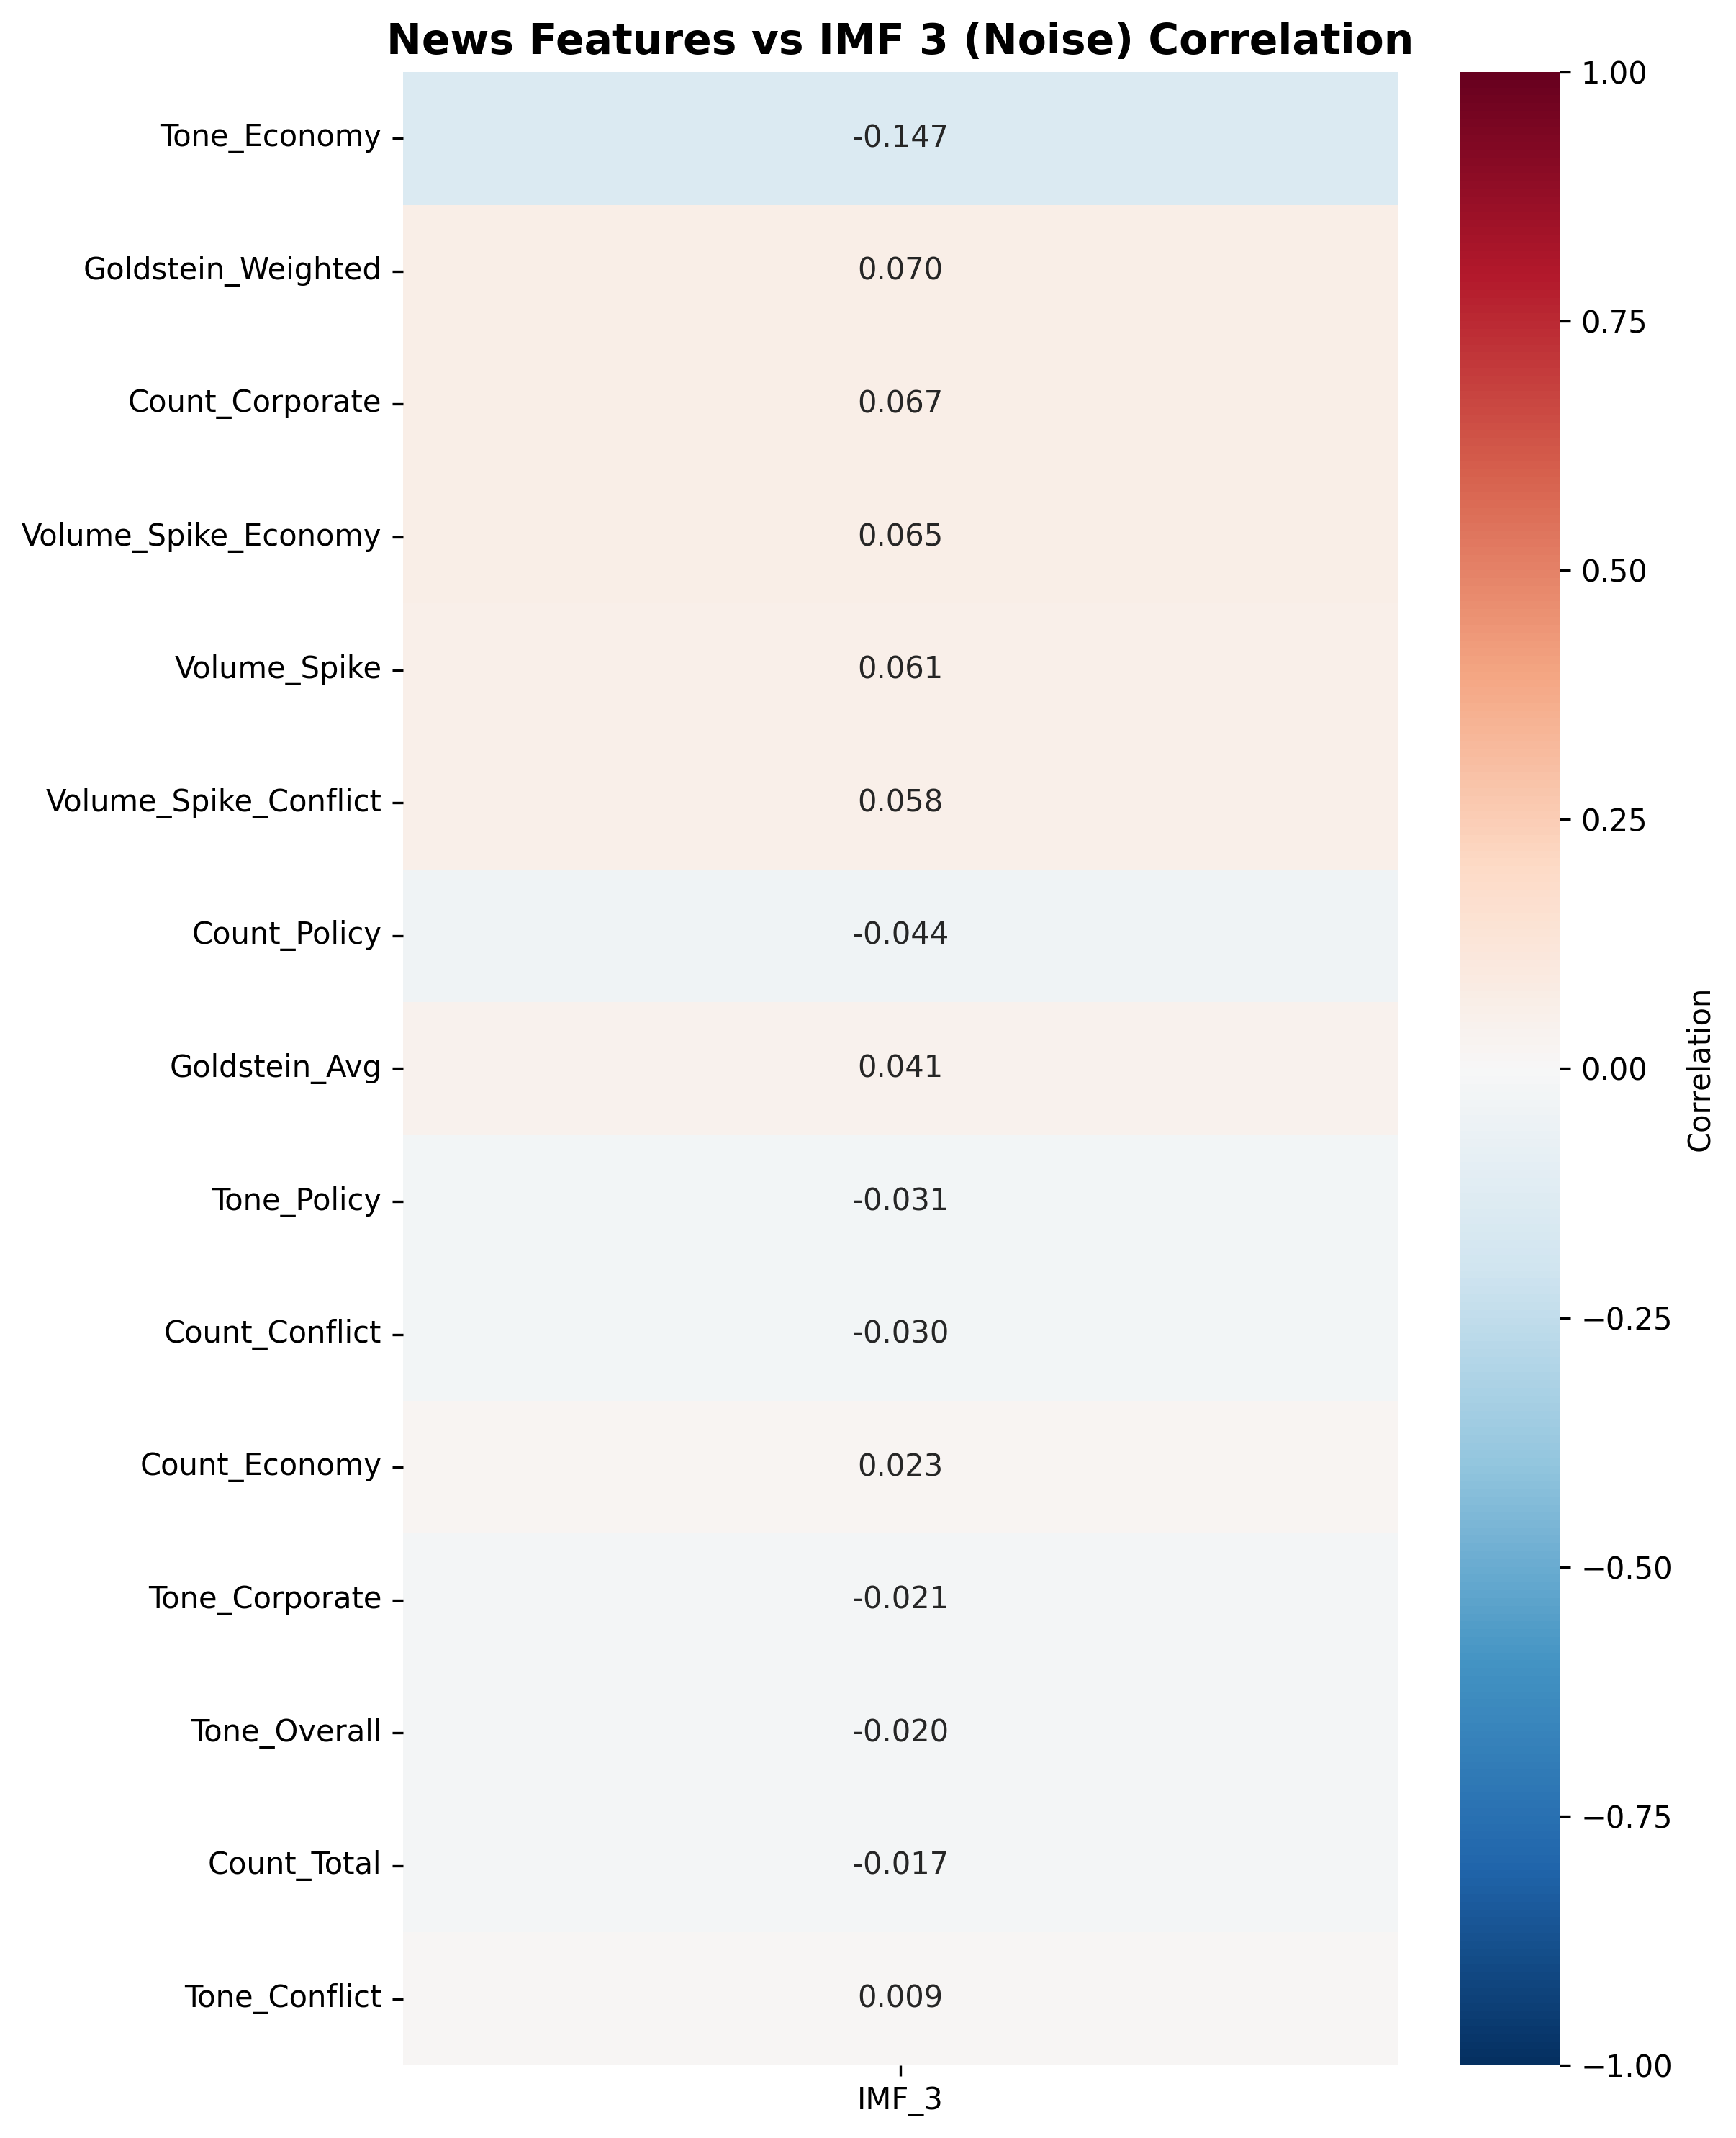
\includegraphics[width=\linewidth,height=3.15cm,keepaspectratio]{phase_b_heatmap.png}
\end{minipage}
\vspace{0.8mm}
\begin{tcolorbox}[colback=PosterSoft,colframe=PosterLine,boxrule=0.4pt,arc=1.6mm,left=1mm,right=1mm,top=0.6mm,bottom=0.6mm]
{\fontsize{6}{6.8}\selectfont Key insight: raw aggregates look random, but filtered themes recover structure.}
\end{tcolorbox}
\end{posterbox}
\end{minipage}\hfill
\begin{minipage}[t]{0.492\textwidth}
\begin{posterbox}
\sectionlabel{2. VMD + STATS}
\boxtitle{VMD Turns Price into Volatility}
\begin{minipage}[t]{0.52\linewidth}
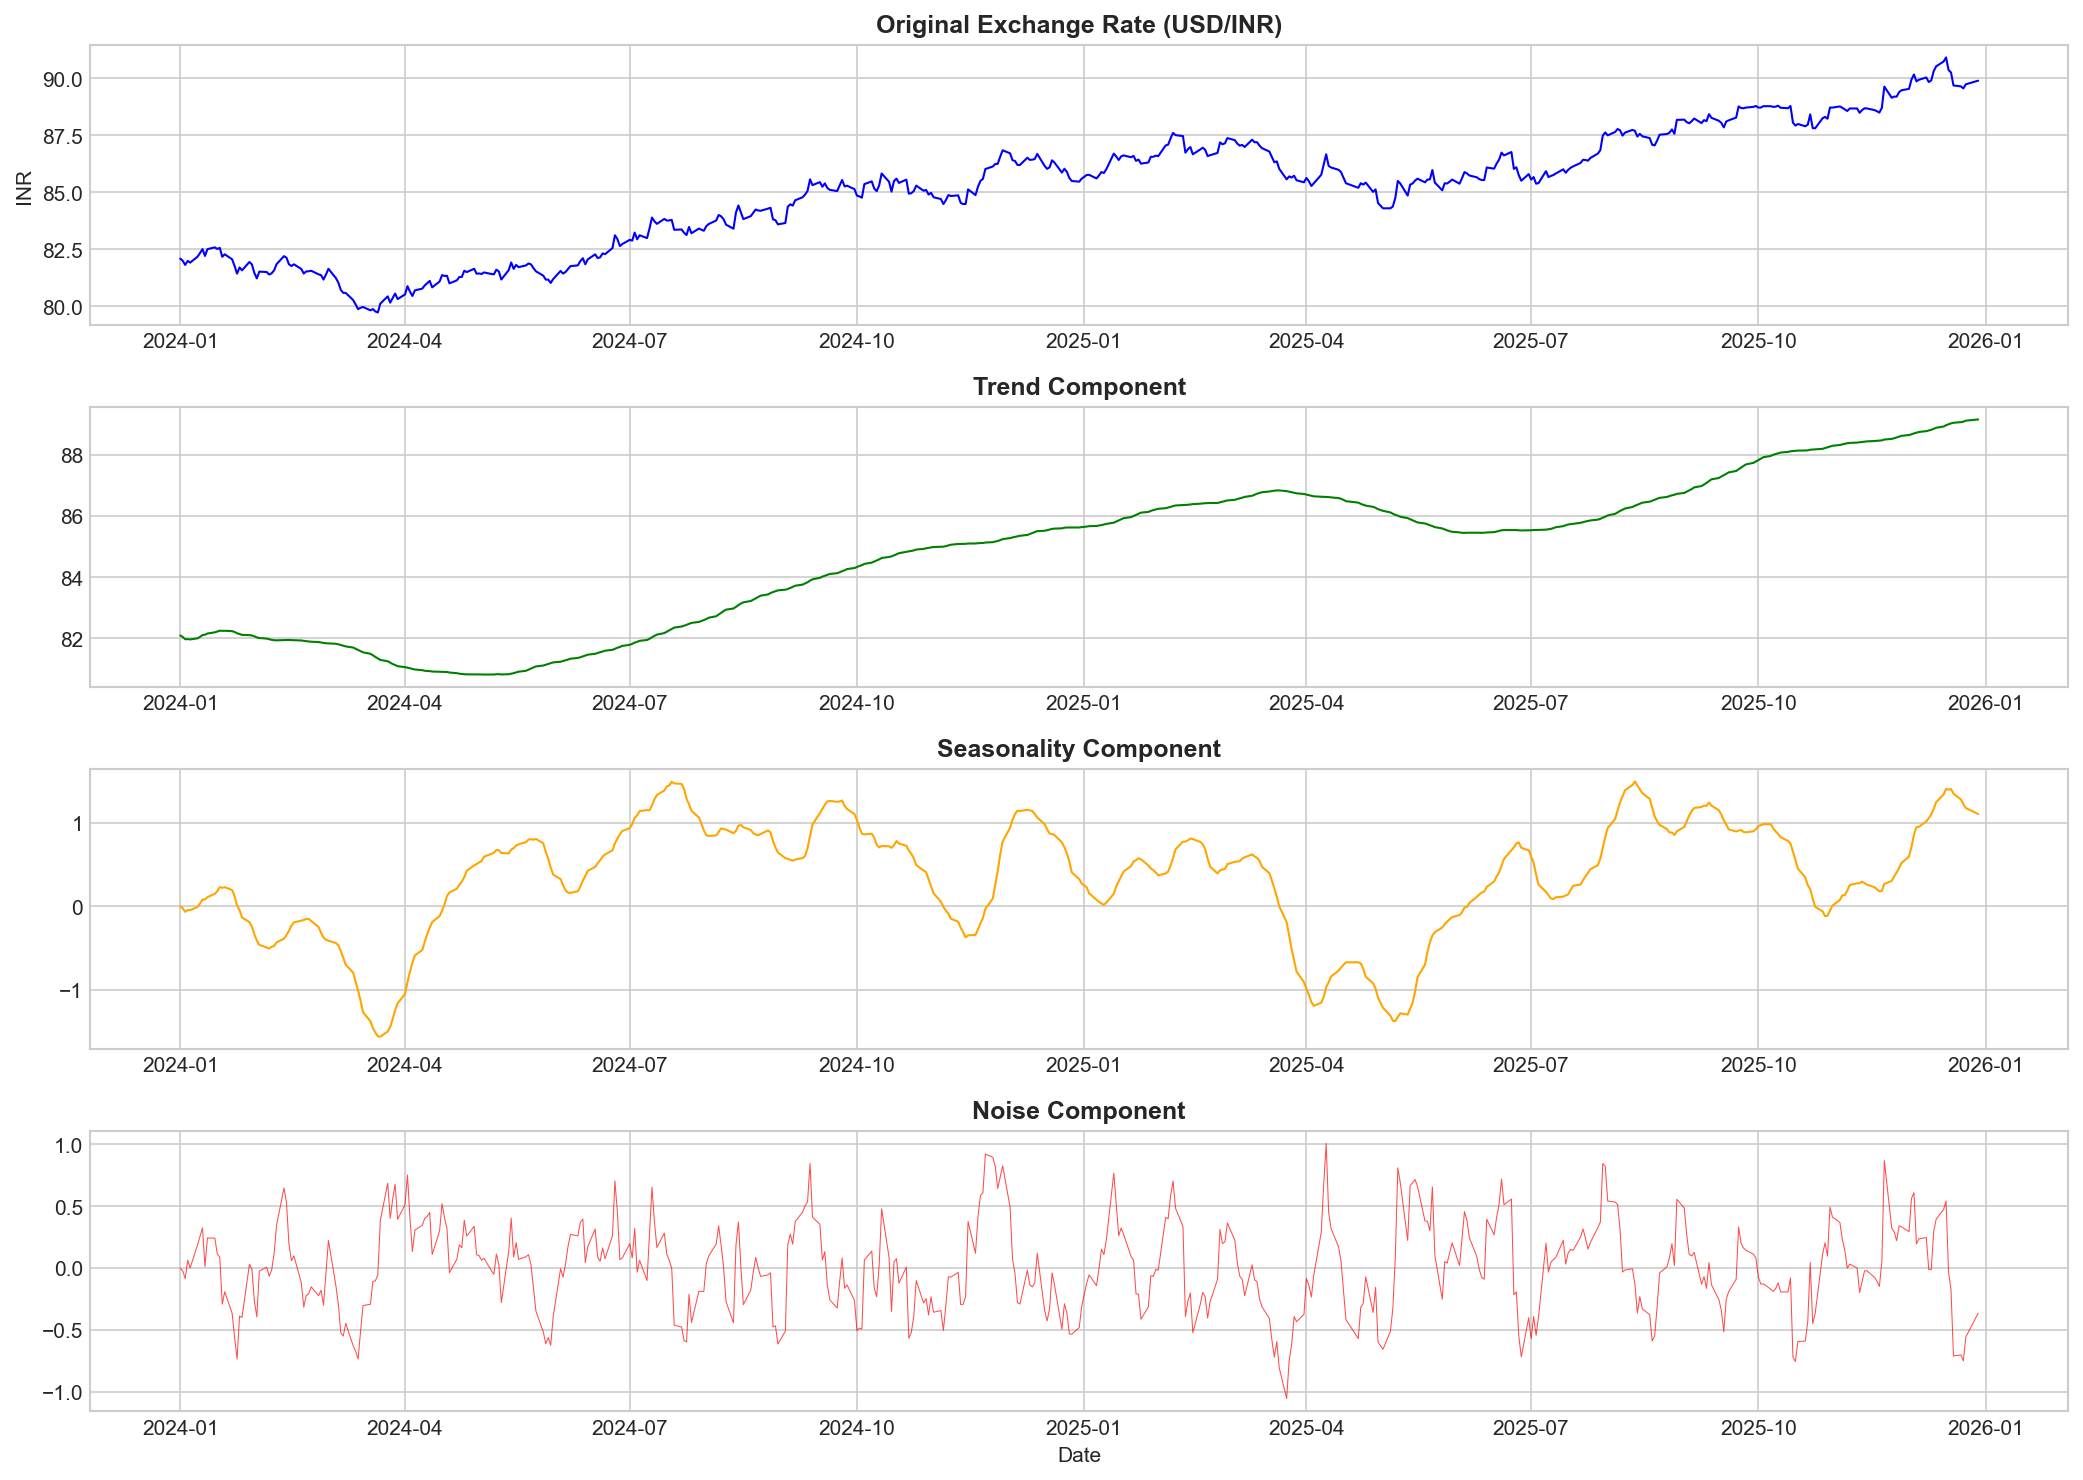
\includegraphics[width=\linewidth,height=2.7cm,keepaspectratio]{ensemble_vmd_decomposition.png}
\end{minipage}\hfill
\begin{minipage}[t]{0.44\linewidth}
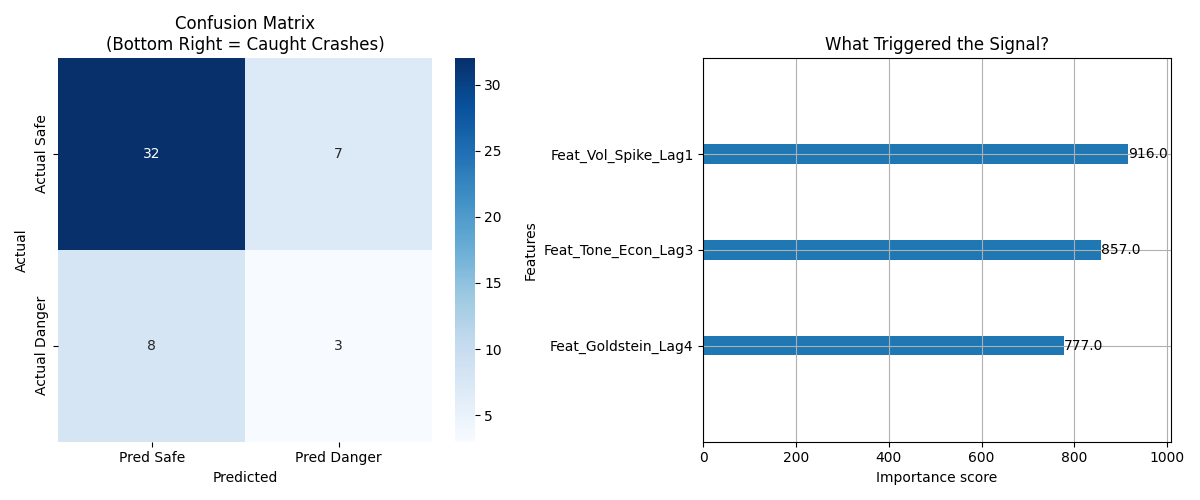
\includegraphics[width=\linewidth,height=2.7cm,keepaspectratio]{phase_c_classifier.png}
\end{minipage}
\vspace{0.7mm}
\begin{itemize}[leftmargin=3.5mm,itemsep=0.4mm,topsep=0.4mm]
\item VMD targets \textbf{IMF3}, the high-frequency part of USD/INR.
\item Phase B uses \textbf{Economy}, \textbf{Conflict}, \textbf{Policy}, and \textbf{Corporate} themes.
\item \textbf{Tone\_Economy = -0.147}; Phase-C reaches \textbf{40\% precision} and \textbf{52\% recall}.
\end{itemize}
\end{posterbox}
\end{minipage}

\vspace{2mm}

\noindent
\begin{minipage}[t]{0.492\textwidth}
\begin{posterbox}
\sectionlabel{3. MONTE CARLO}
\boxtitle{Monte Carlo as a Randomness Check}
\centering
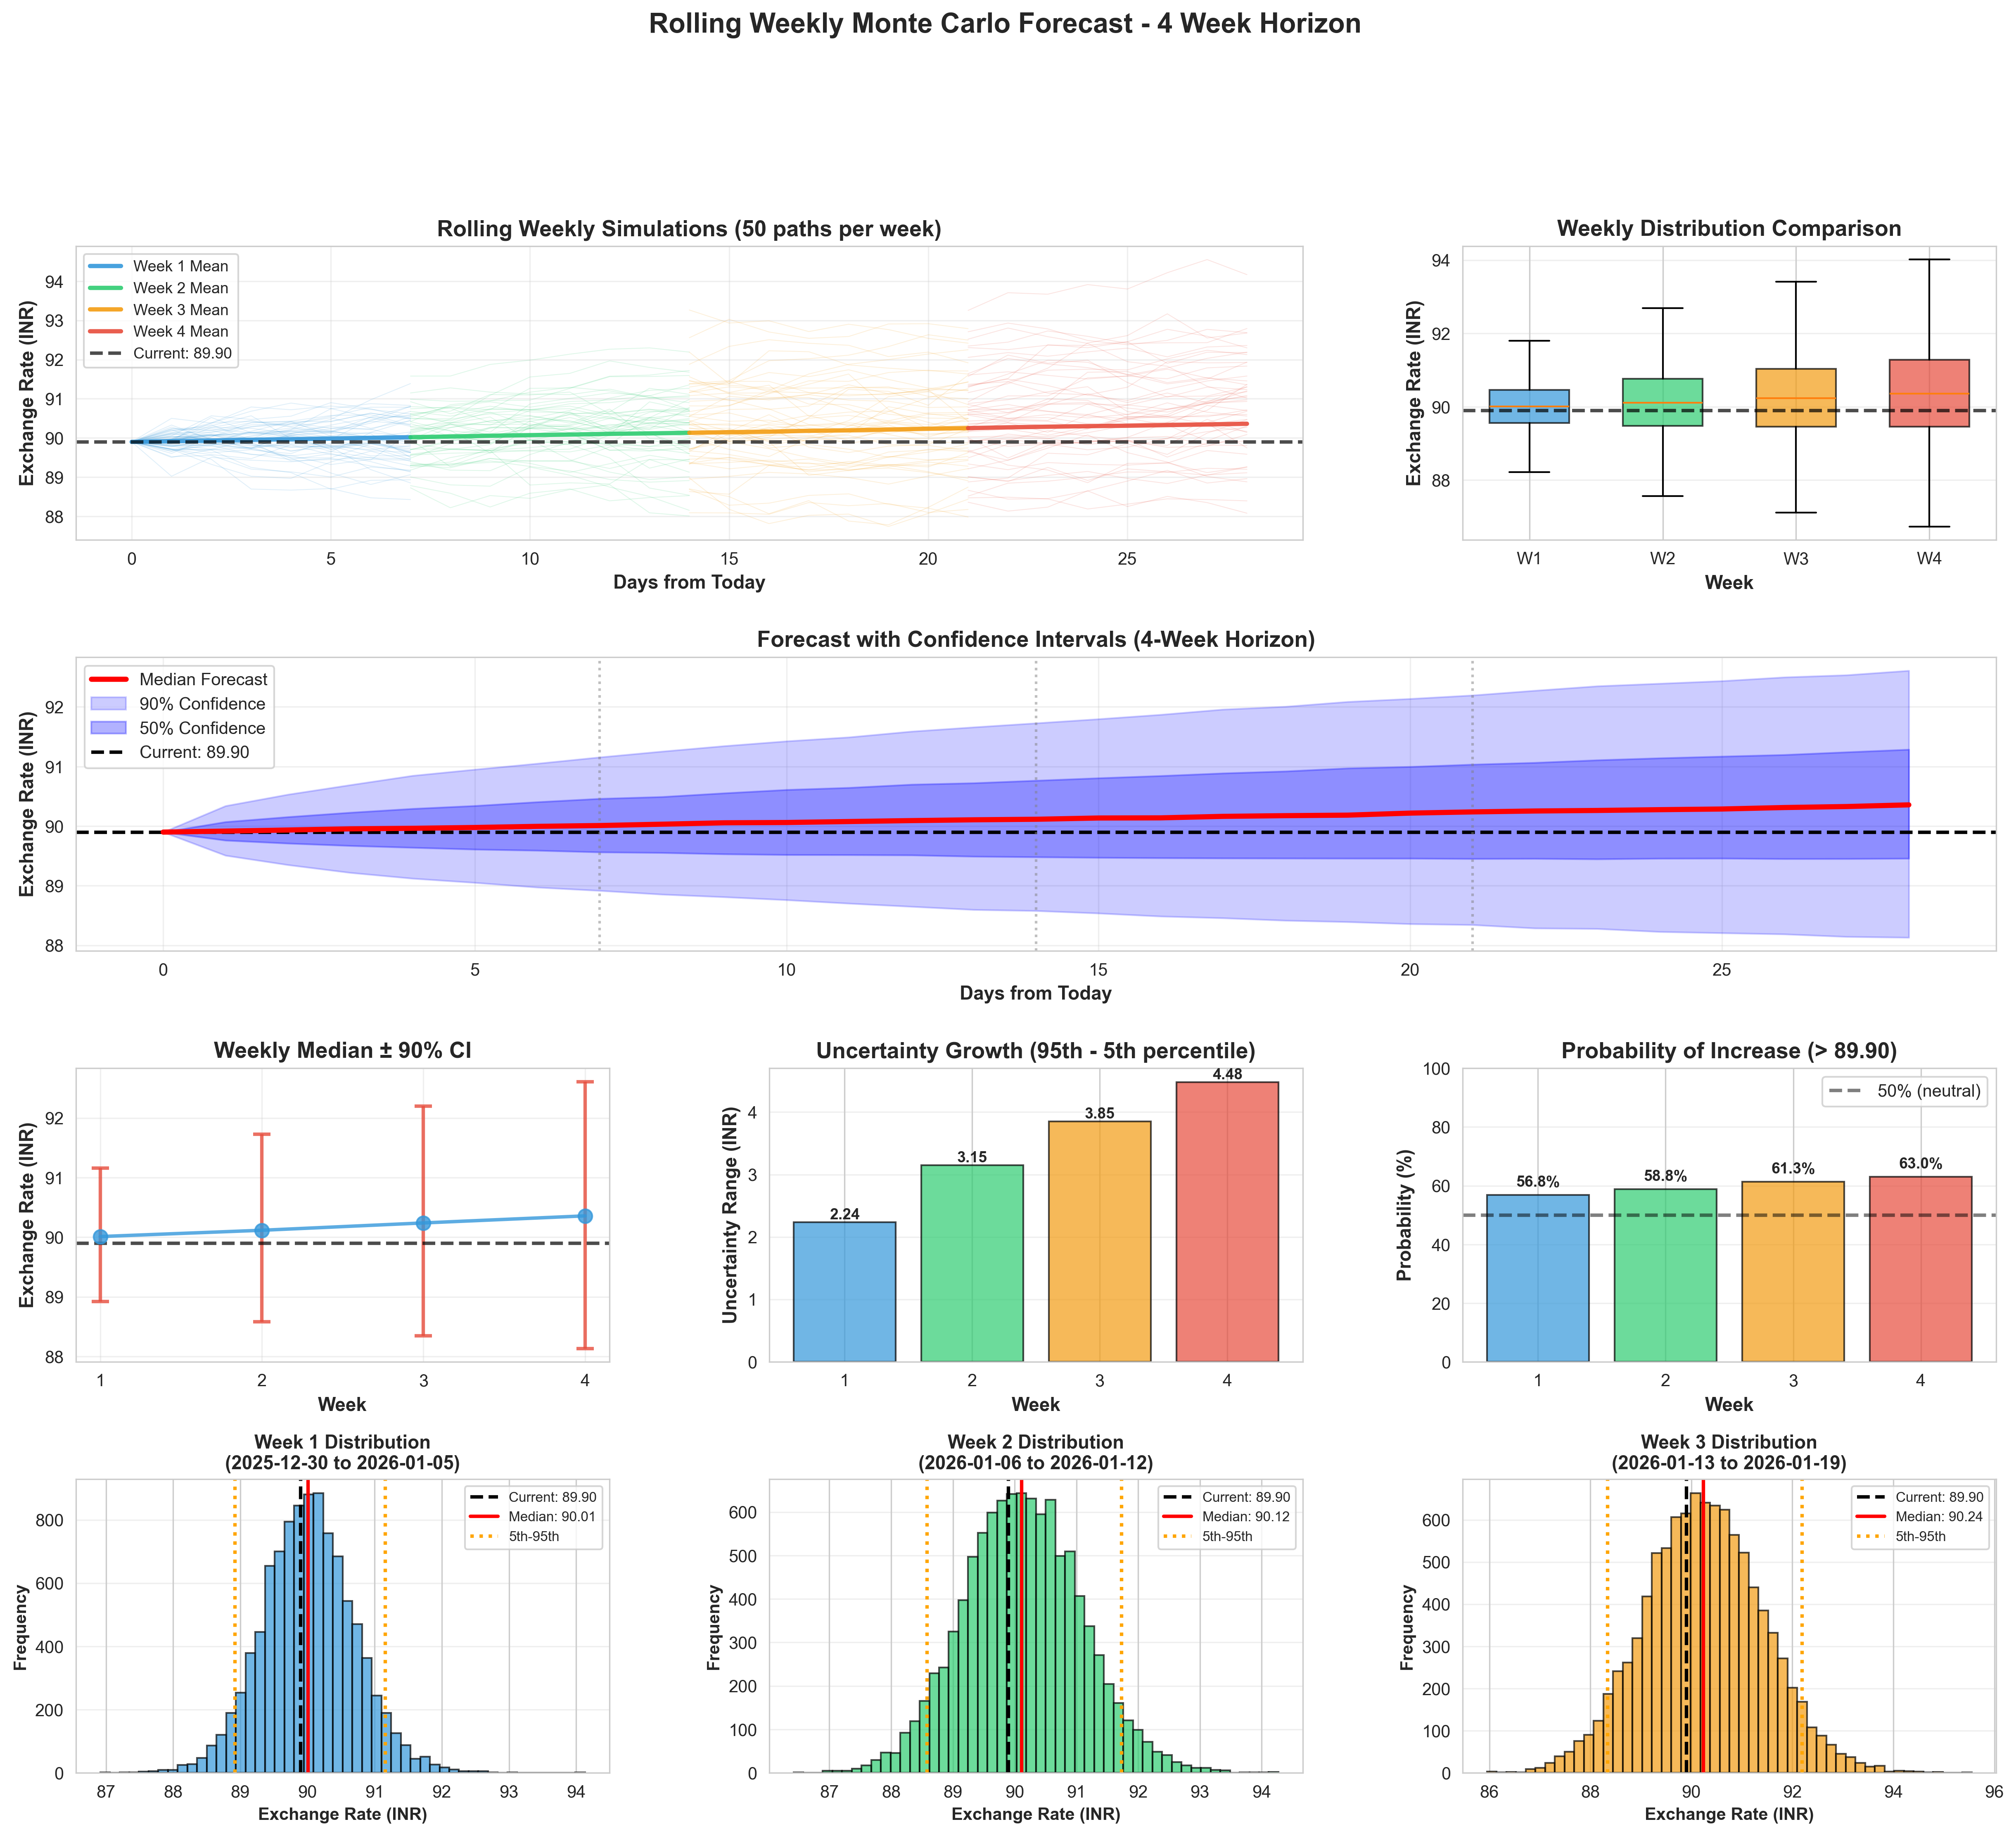
\includegraphics[width=\linewidth,height=2.7cm,keepaspectratio]{monte_carlo_weekly.png}
\par
\vspace{0.7mm}
\begin{itemize}[leftmargin=3.5mm,itemsep=0.4mm,topsep=0.4mm]
\item Monte Carlo works best as a \textbf{risk engine}, not a point predictor.
\item Best 30-day setup: regime switching with median \textbf{90.370} and std \textbf{1.336}.
\end{itemize}
\end{posterbox}
\end{minipage}\hfill
\begin{minipage}[t]{0.492\textwidth}
\begin{posterbox}
\sectionlabel{4. GDELT AGENTS}
\boxtitle{Bounded GDELT LLM Overlay}
\begin{minipage}[t]{0.54\linewidth}
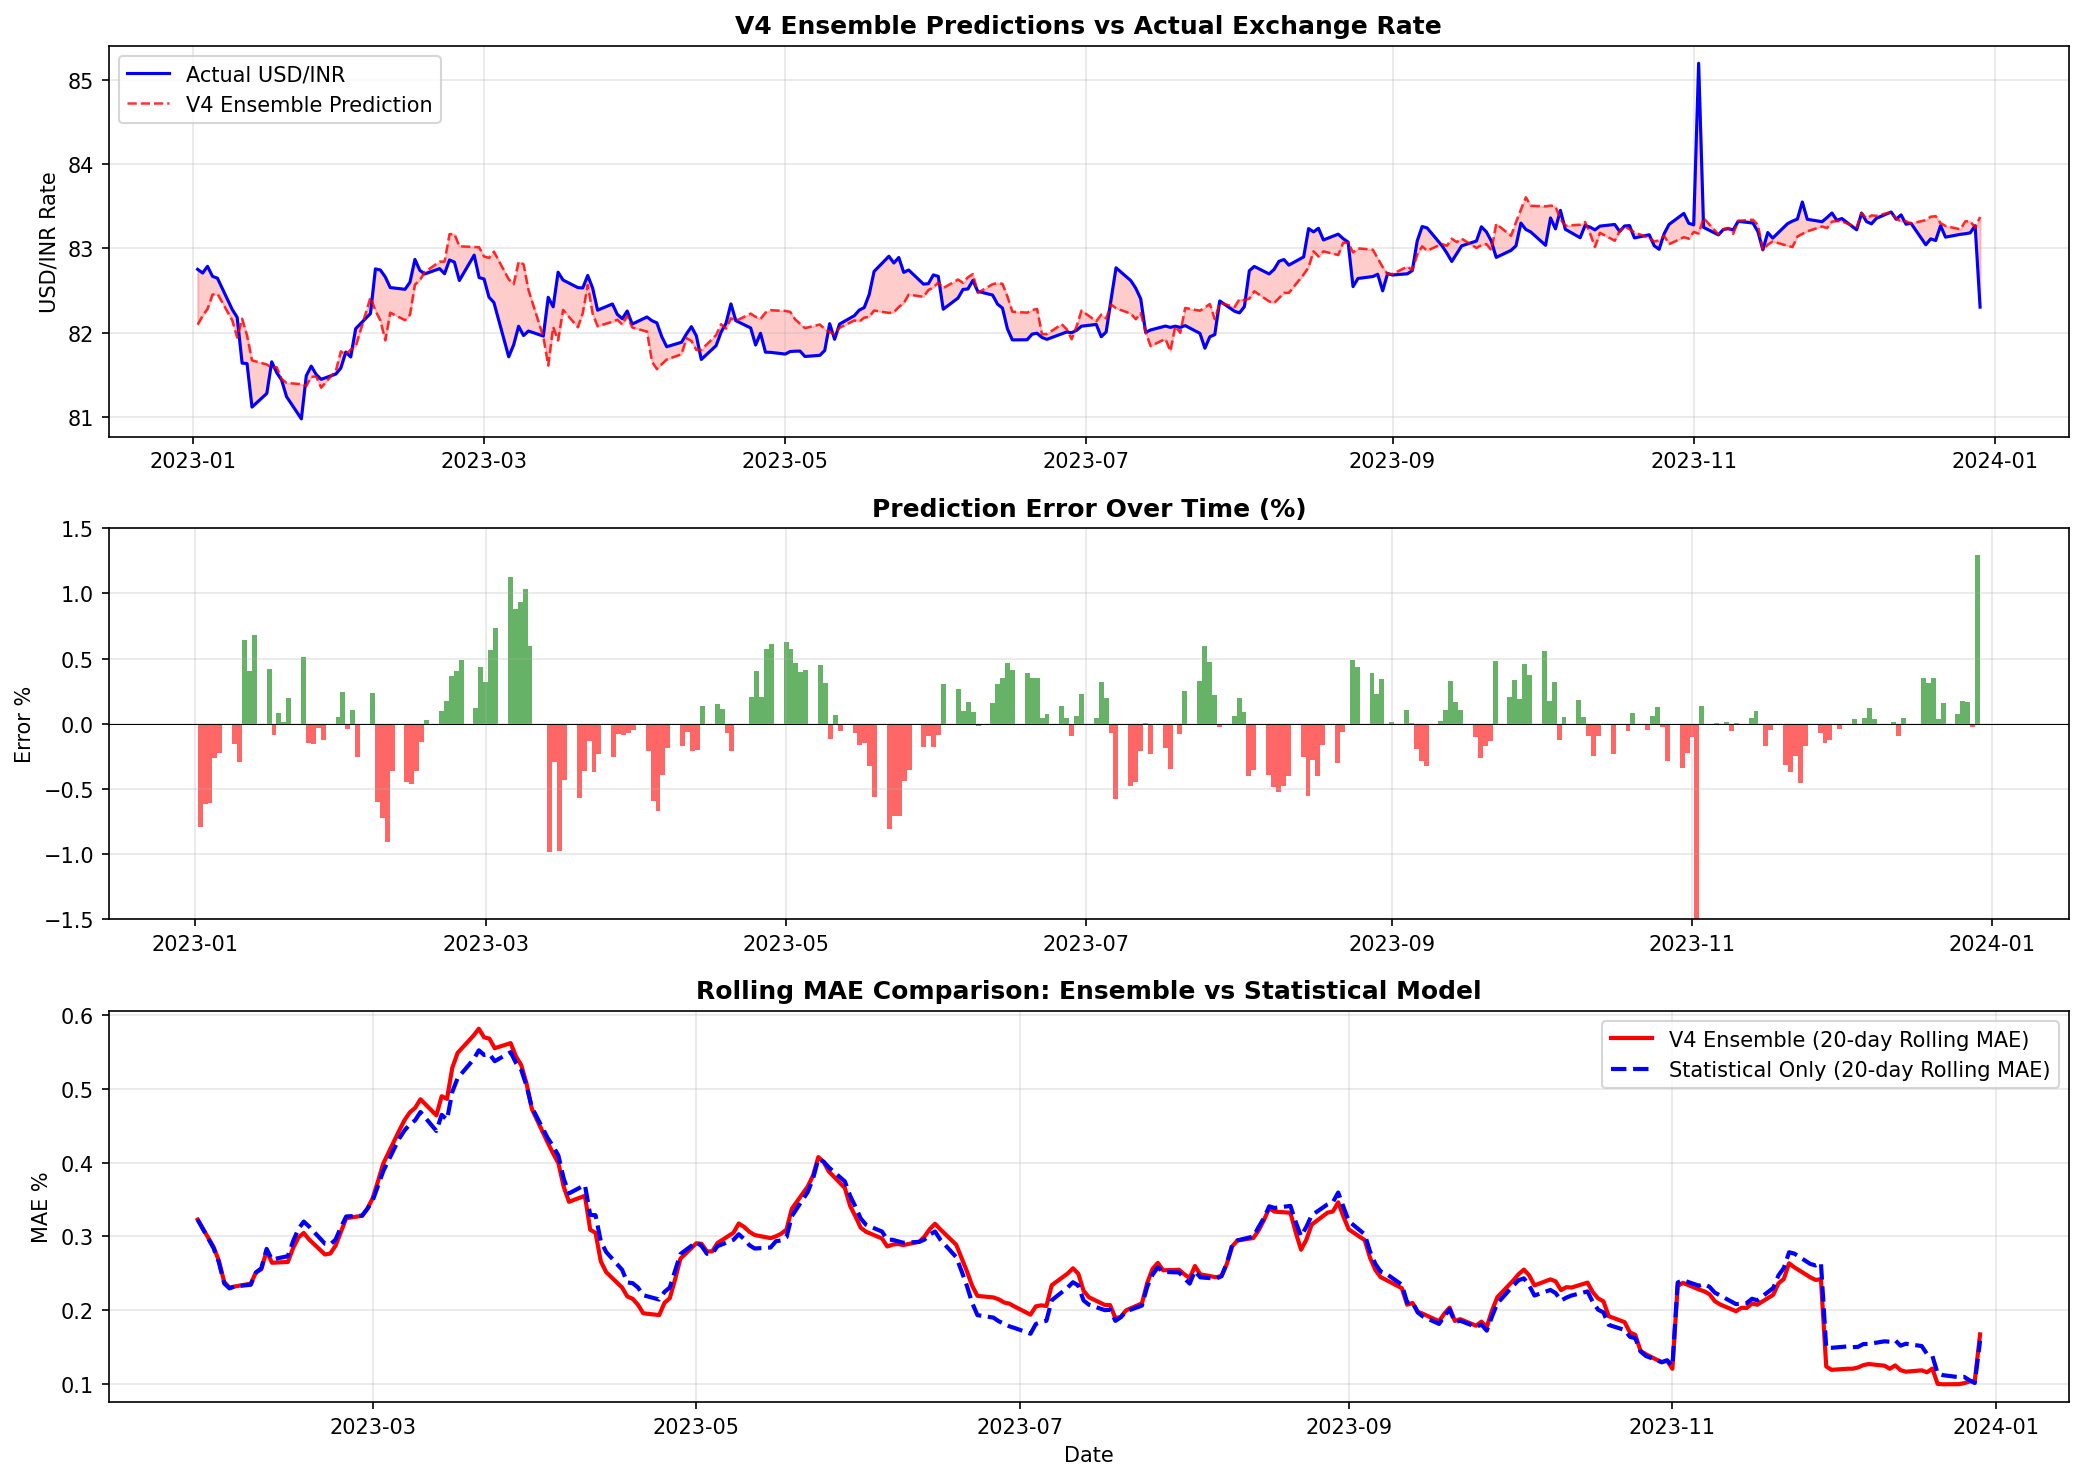
\includegraphics[width=\linewidth,height=2.2cm,keepaspectratio]{gemini_v4_comparison.png}
\end{minipage}\hfill
\begin{minipage}[t]{0.42\linewidth}
\begin{tcolorbox}[colback=PosterSoft,colframe=PosterLine,boxrule=0.4pt,arc=1.4mm,left=0.7mm,right=0.7mm,top=0.6mm,bottom=0.5mm]
{\color{PosterBlue}\bfseries\fontsize{6.2}{6.4}\selectfont V4 ACCURACY TABLE\par}
\vspace{0.4mm}
\centering
\fontsize{5.6}{6.3}\selectfont
\resizebox{\linewidth}{!}{
\begin{tabular}{@{}lccc@{}}
\toprule
Model & Days & MAE & Dir. \\
\midrule
V3 hybrid & 240 & 0.2741\% & 61.25\% \\
V4 hybrid & 240 & \textbf{0.2695\%} & \textbf{64.17\%} \\
V4 Jan live & 21 & 0.3216\% & 57.14\% \\
\bottomrule
\end{tabular}
}
\end{tcolorbox}
\end{minipage}
\vspace{0.7mm}
{\fontsize{5.9}{6.7}\selectfont Debiasing improved V4 through symmetric prompts, random order, and adaptive weights.\par}
\end{posterbox}
\end{minipage}

\vspace{2mm}

\noindent
\begin{minipage}[t]{0.492\textwidth}
\begin{posterbox}
\sectionlabel{5. TEPC}
\boxtitle{TEPC: Topology and Chaos Results}
\centering
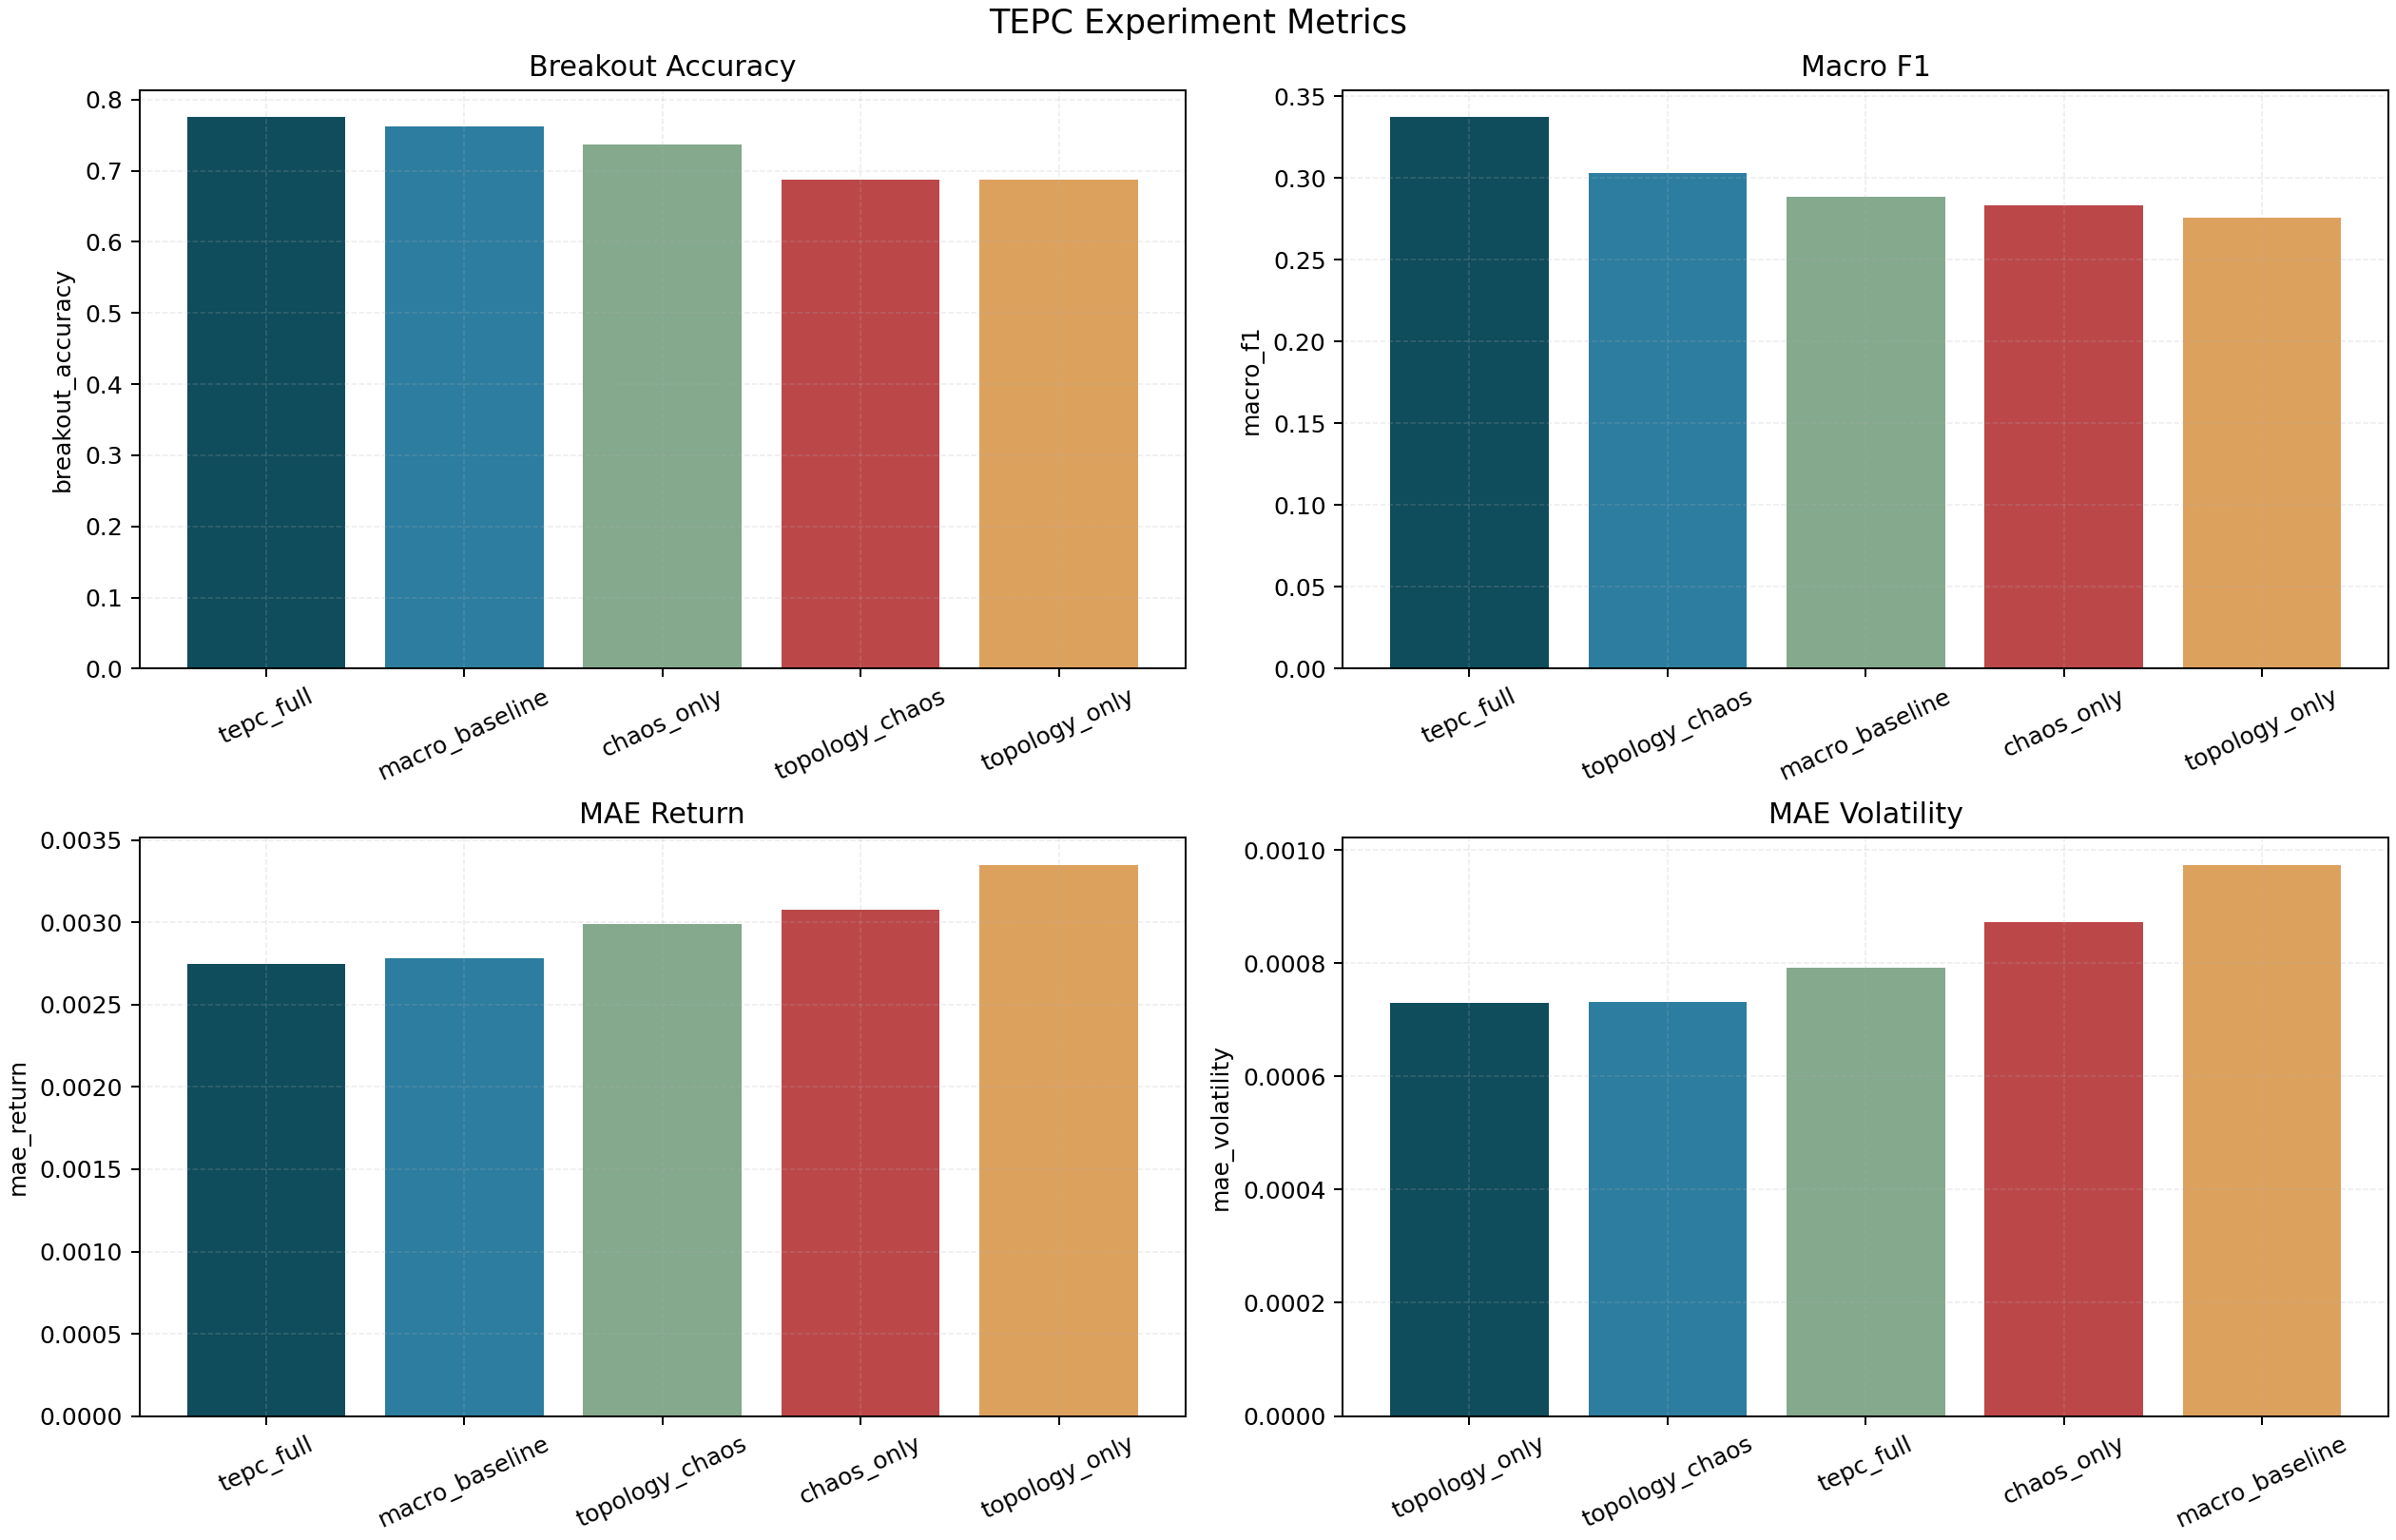
\includegraphics[width=\linewidth,height=2.2cm,keepaspectratio]{tepc_strict_metric_bars.png}
\par
\vspace{0.7mm}
\begin{itemize}[leftmargin=3.5mm,itemsep=0.4mm,topsep=0.4mm]
\item TEPC models USD/INR inside a macro network with DXY, BRENT, GOLD, rates, and sentiment.
\item Graph features and coupled Lorenz chaos features become predictors.
\item \textbf{tepc\_full}: \textbf{77.5\%} breakout accuracy, \textbf{0.337} macro-F1, \textbf{0.002746} MAE return. Live \textbf{chaos\_only} reaches \textbf{80\%}.
\end{itemize}
\end{posterbox}
\end{minipage}\hfill
\begin{minipage}[t]{0.492\textwidth}
\begin{posterbox}
\sectionlabel{6. HYBRID TAKEAWAY}
\boxtitle{TEPC + LLM Hybrid Results}
\begin{minipage}[t]{0.54\linewidth}
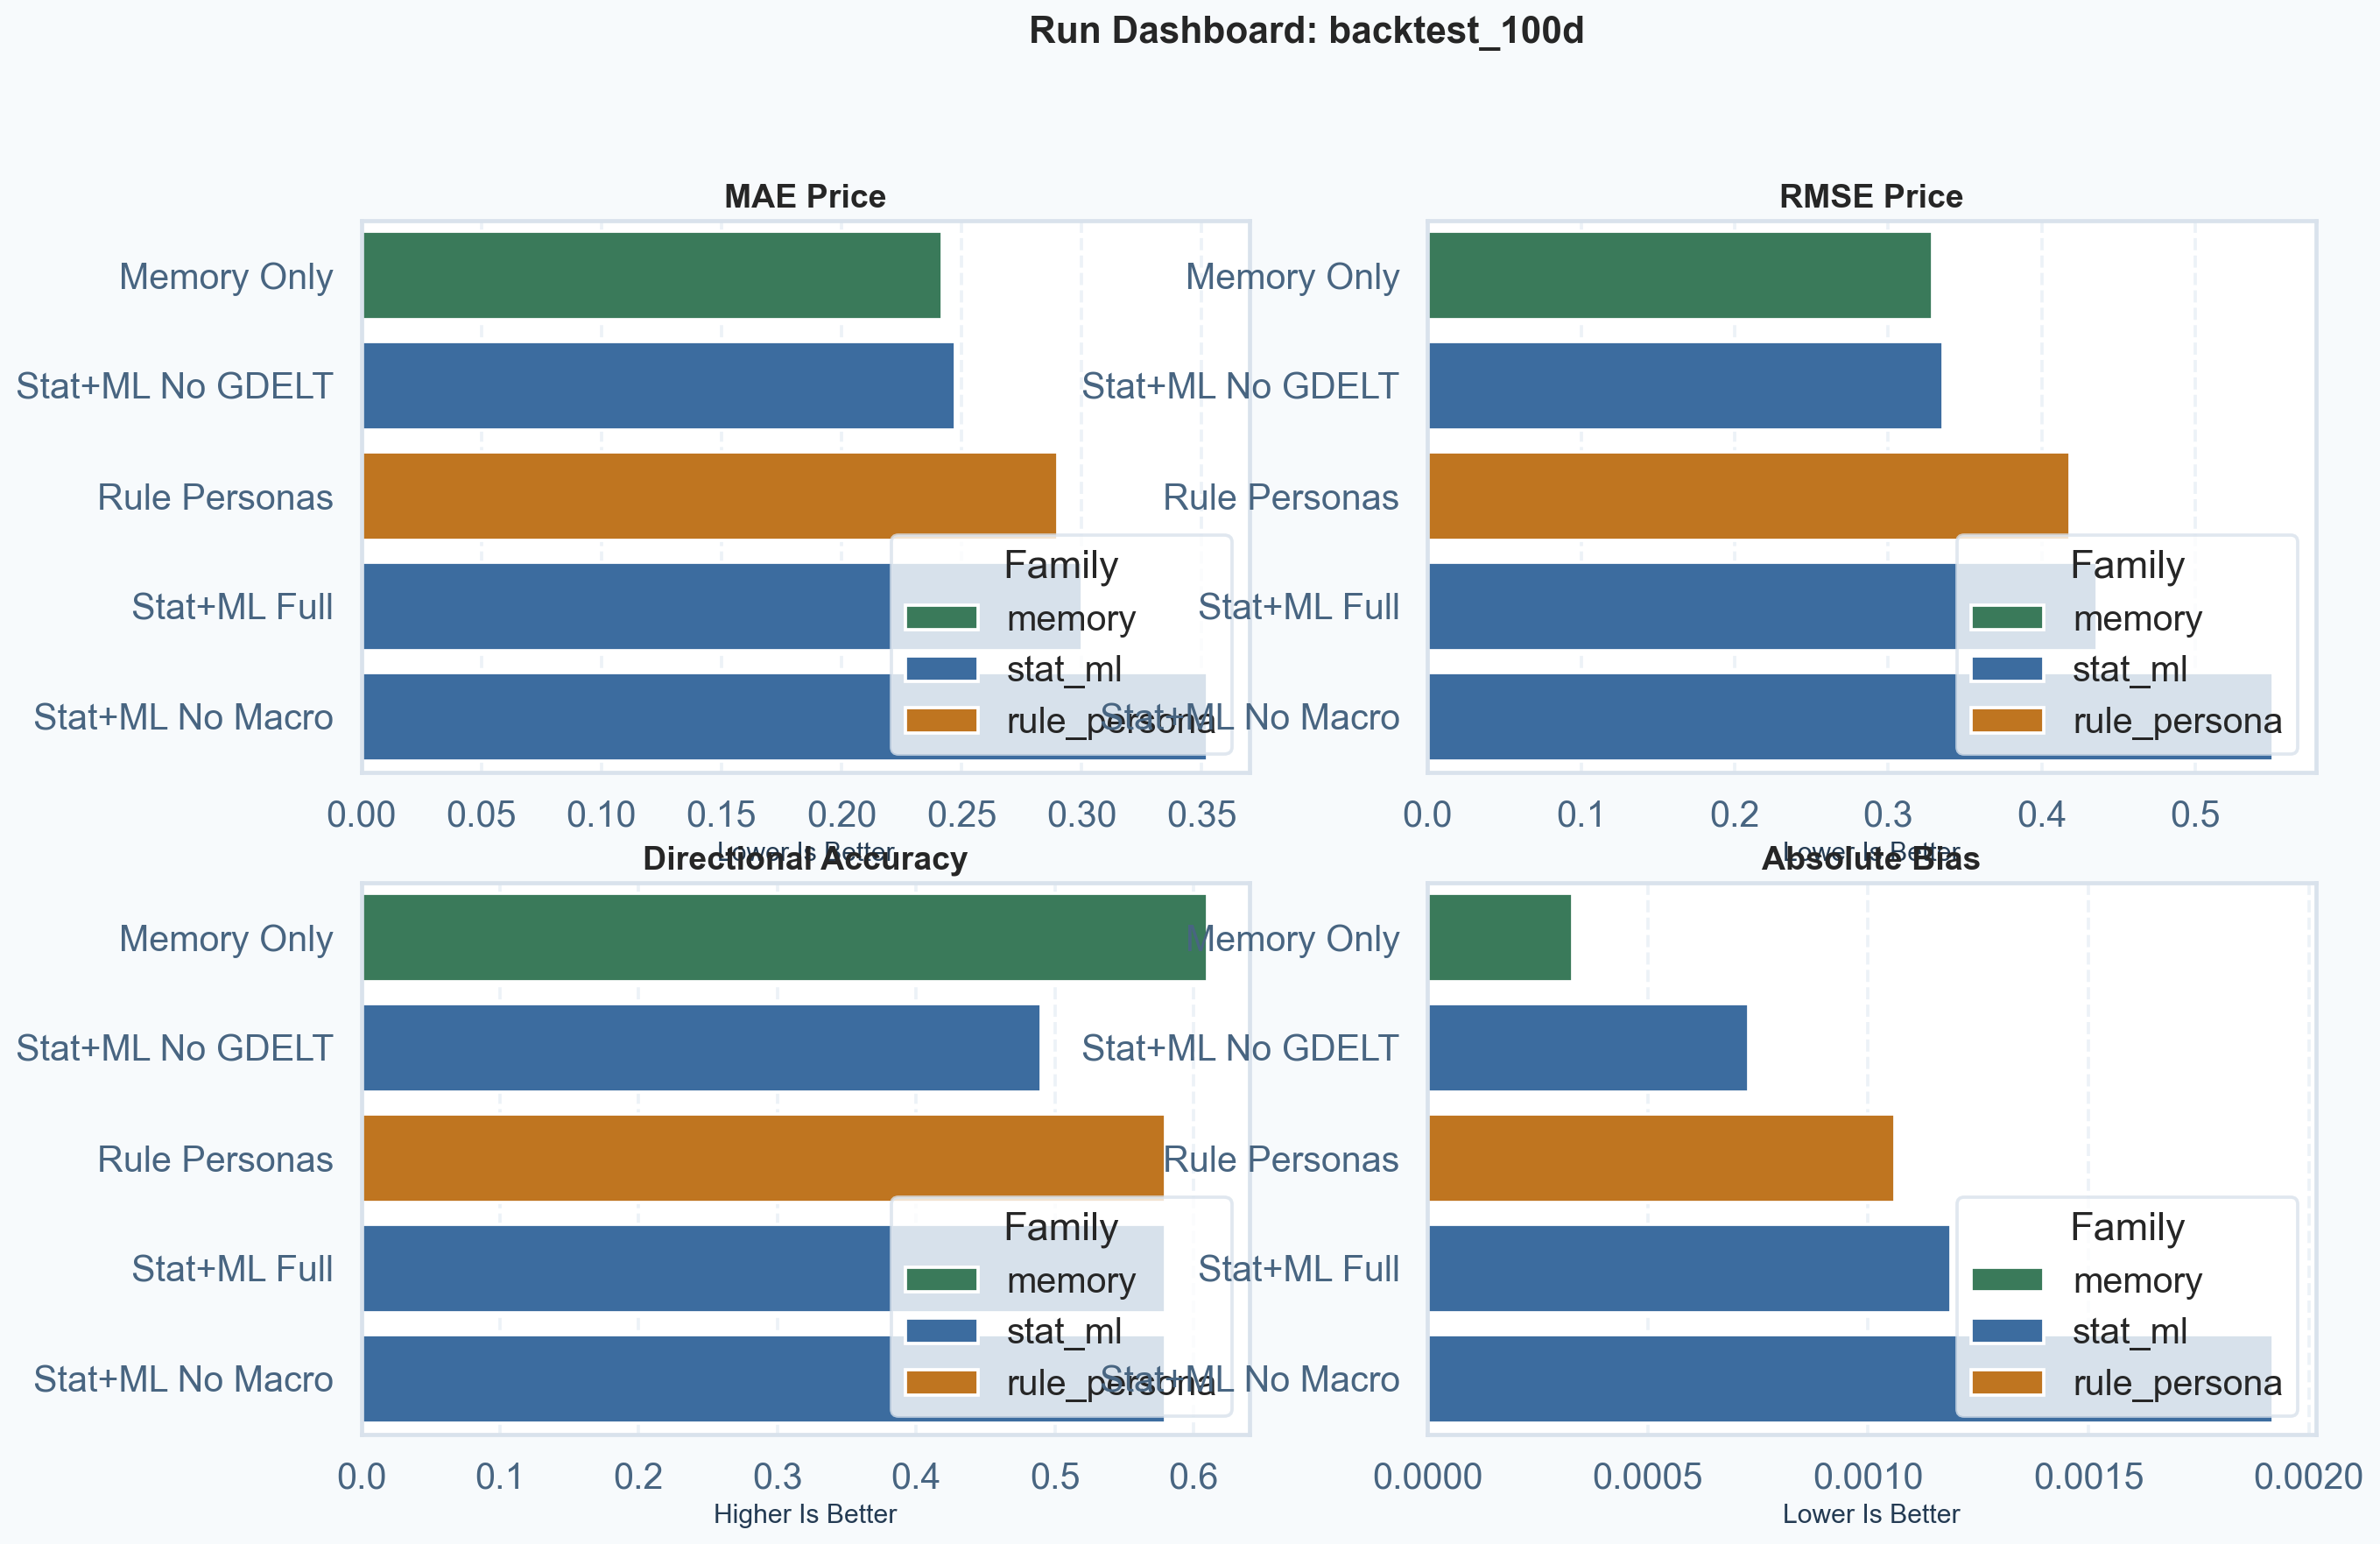
\includegraphics[width=\linewidth,height=2.15cm,keepaspectratio]{final_phase_dashboard_100d.png}
\end{minipage}\hfill
\begin{minipage}[t]{0.42\linewidth}
\begin{tcolorbox}[colback=PosterSoft,colframe=PosterLine,boxrule=0.4pt,arc=1.4mm,left=0.7mm,right=0.7mm,top=0.6mm,bottom=0.5mm]
{\color{PosterBlue}\bfseries\fontsize{6.2}{6.4}\selectfont HYBRID TABLE\par}
\vspace{0.4mm}
\centering
\fontsize{5.3}{6.1}\selectfont
\resizebox{\linewidth}{!}{
\begin{tabular}{@{}lccc@{}}
\toprule
Model & Window & Acc. & Error \\
\midrule
Memory-only & 100d & 61.0\% dir. & 0.2421 price \\
Gemini 2.5 & 100d & 58.0\% dir. & 0.2726 price \\
TEPC full & 80d & 77.5\% brk. & 0.002746 ret. \\
TEPC blend & 80d & \textbf{78.75\% brk.} & \textbf{0.002695 ret.} \\
\bottomrule
\end{tabular}
}
\end{tcolorbox}
\end{minipage}
\vspace{0.7mm}
{\fontsize{5.9}{6.7}\selectfont LLMs help most with structured market memory, and TEPC adds regime signal on top.\par}
\end{posterbox}
\end{minipage}

\vspace{1.0mm}
\hrule height 0.8pt
\vspace{0.8mm}
{\fontsize{5.45}{5.9}\selectfont \textbf{Final Message:} best results come from \textbf{VMD + GDELT filtering + bounded LLM overlays + TEPC topology/chaos features}, not from a larger black-box model.\par}

\end{document}
